\subsection{Minimization of Feeder Real Power Scenario}

The goal of this experiment was to test the effectiveness of the \emph{LinDist3Flow} model in an OPF formulation, with \textbf{A1} - \textbf{A2} applied to \eqref{eq:mag_17} - \eqref{eq:pow_13} as outlined in Section \ref{subsec:analysis_nominal} (resulting in Eqs. \eqref{eq:pow_12_lin} - \eqref{eq:mag_19_lin}) .  The objective of the OPF was to control DER real and reactive power resources to minimize feeder head real power, subject to voltage magnitude and DER inverter capacity constraints.

Minimization of feeder head real power was chosen as the objective of \eqref{eq:OPF1} as it is possible to compare results to those determined via convex relaxation techniques and semidefinite programming, outlined in \cite{dall2012optimization} - \cite{dall2013distributed} (we henceforth refer to these results as ``SDP").  In this scenario, we assumed constant power loads where $a_{0,n}^{\phi} = 1$ and $a_{1,n}^{\phi} = 0 \text{ } \forall n \in H$. We define the OPF that employs the \textit{LinDist3Flow} model as:
\begin{equation}
\begin{aligned}
	& \underset{u_{n}^{\phi},v_{n}^{\phi},y_{n}^{\phi},P_{n}^{\phi},Q_{n}^{\phi}} {\text{minimize}} & & \sum_{\phi \in \{ a,b,c\}} P_{0}^{\phi} \\
    & \text{subject to} & & \eqref{eq:pow_12_lin} - \eqref{eq:mag_19_lin}, \quad \underline{y} \le y_{n}^{\phi} \le \overline{y}, \\
    & & & \left| w_{n}^{\phi} \right| \le \overline{w}, \quad \forall n \in H
\end{aligned}
\label{eq:OPF1}
\end{equation}

% Minimization of feeder head real power was chosen as the objective of \eqref{eq:OPF1} as it is possible to compare to compare the results of \eqref{eq:OPF1} to those determined via convex relaxation techniques and semidefinite programming, outlined in \cite{dall2012optimization} - \cite{dall2013distributed} (we henceforth refer to these results as ``SDP").  In this scenario, we assume constant power loads where $a_{0,n}^{\phi} = 1$ and $a_{1,n}^{\phi} = 0 \text{ } \forall k \in H$.

A comparison between the SDP and the OPF of \eqref{eq:OPF1} is shown in Fig. \ref{fig:s1}, with Fig. \ref{fig:s1sdp} showing the voltage magnitude profile using the SDP optimal control (note that the SDP achieved a rank 1 solution), and Fig. \ref{fig:s1lin} showing the voltage magnitude profile obtained from applying control inputs determined from \eqref{eq:OPF1}.  Though there is a visible difference in the voltage profiles derived in each case, both control formulations deployed DER resources to bring voltages to within acceptable limits.  Interestingly, while the optimal control given by the SDP and \eqref{eq:OPF1} had the same real parts (DER real power output), the imaginary parts (DER reactive output) were different, leading to different voltage magnitudes. The optimal cost, computed as $\sum_{\phi \in \{ a,b,c\}} P_{0}^{\phi}$, was 0.83732 p.u. for the uncontrolled case, 0.27634 p.u. for the SDP case, and 0.27688 p.u. for the case of \eqref{eq:OPF1}, a difference of 0.2 \%.

% \begin{figure}[t]
% \centering
% \begin{subfigure}[b]{0.49\textwidth}
% 	\centering
% 	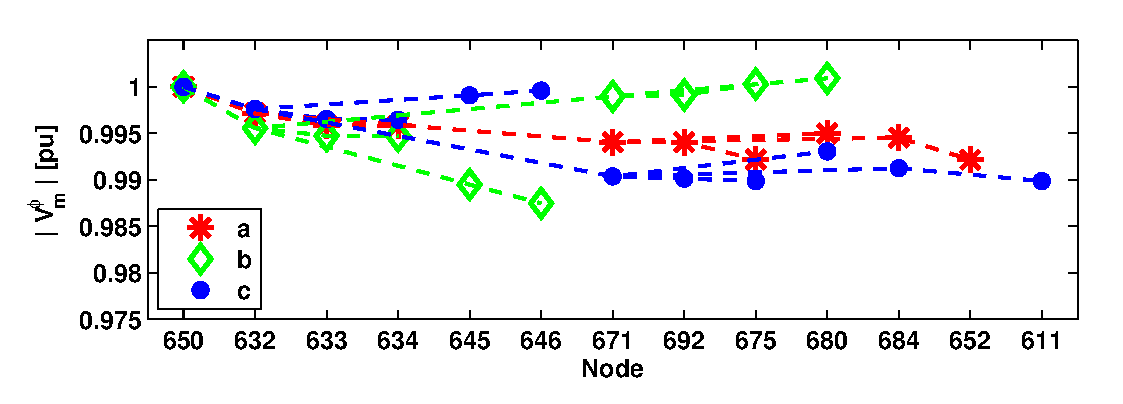
\includegraphics[width=\textwidth]{s1sdp.eps}
% 	\caption{Voltage profile of feeder with SDP control.}
% 	\label{fig:s1sdp}
% \end{subfigure}
% \\
% \begin{subfigure}[b]{0.49\textwidth}
% 	\centering
% 	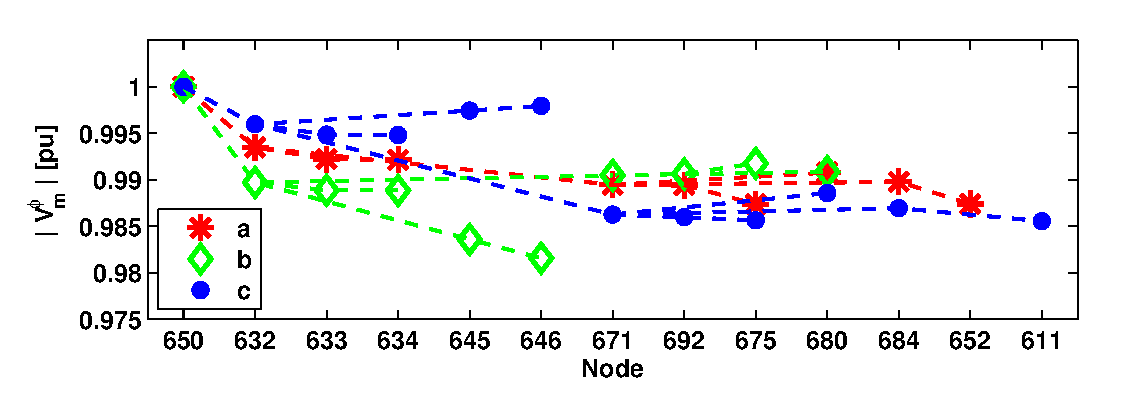
\includegraphics[width=\textwidth]{s1lin.eps}
% 	\caption{Voltage profile of feeder with our OPF control.}
% 	\label{fig:s1lin}
% \end{subfigure}
% \caption{Voltage profiles for SDP and our OPF.}
% \label{fig:s1}
% \end{figure}

% \begin{figure}[t]
% 	\centering
% 	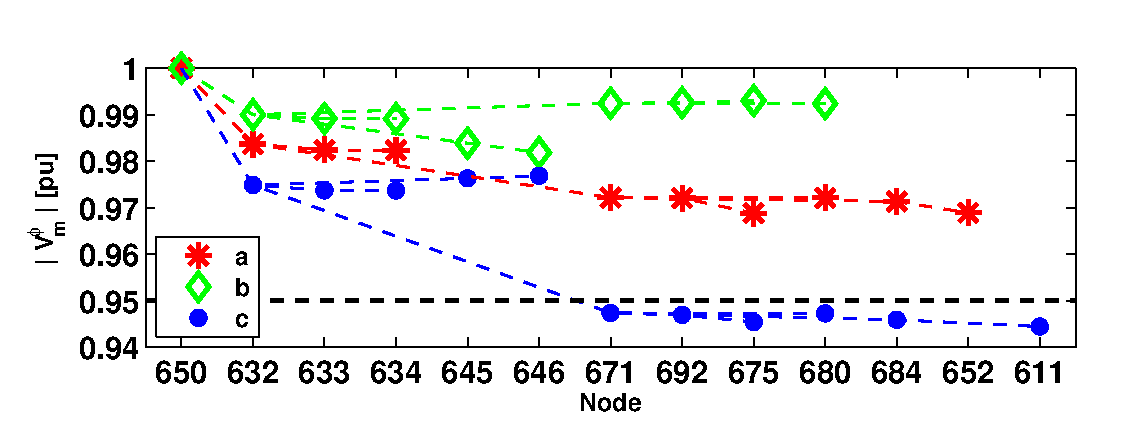
\includegraphics[width=0.49\textwidth]{s2bc.eps}
% 	\caption{Voltage profile of IEEE 13 node feeder with zero control.}
% 	\label{fig:s2bc}
%   \begin{subfigure}[b]{0.49\textwidth}
%       \centering
%       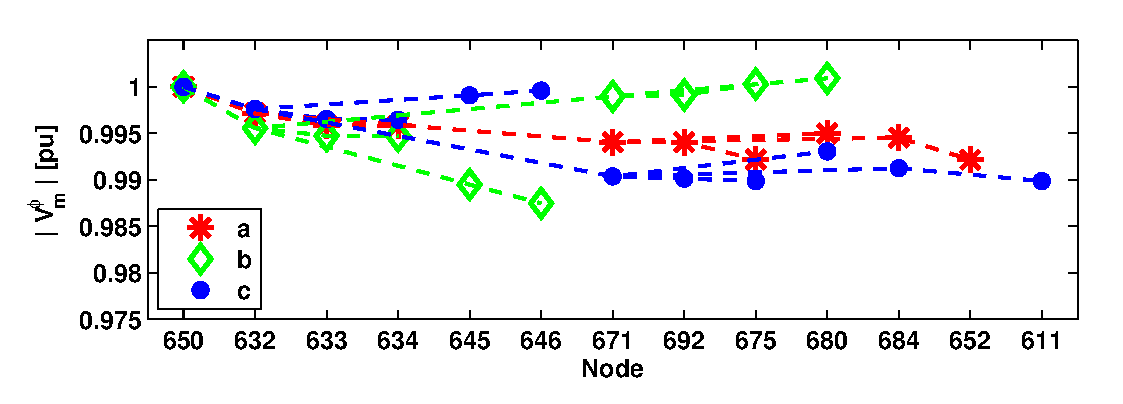
\includegraphics[width=\textwidth]{s1sdp.eps}
%       \caption{Voltage profile of IEEE 13 node feeder with SDP control.}
%       \label{fig:s1sdp}
%   \end{subfigure}
%   \\
%   \begin{subfigure}[b]{0.49\textwidth}
%       \centering
%       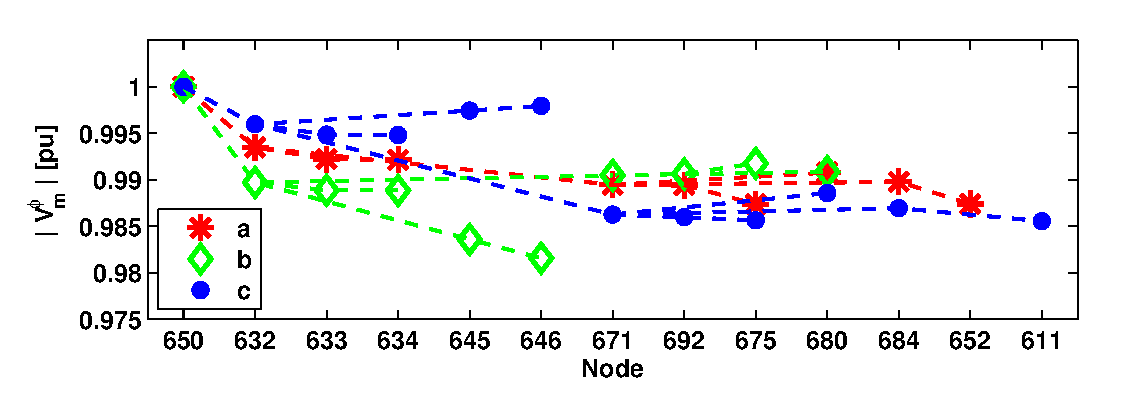
\includegraphics[width=\textwidth]{s1lin.eps}
%       \caption{Voltage profile of IEEE 13 node feeder with control from \eqref{eq:OPF1}}
%       \label{fig:s1lin}
%   \end{subfigure}
%   \caption{Comparison of voltage profiles for feeder head real power minimization simulation.}
%   \label{fig:s1}
%   \begin{subfigure}[b]{0.49\textwidth}
%       \centering
%       \includegraphics[width=\textwidth]{s2c1.eps}
%       \caption{Voltage profile of IEEE 13 node feeder with \eqref{eq:OPF2} Case 1 control input.}
%       \label{fig:s2c1}
%   \end{subfigure}
%   \\
%   \begin{subfigure}[b]{0.49\textwidth}
%       \centering
%       \includegraphics[width=\textwidth]{s2c3.eps}
%       \caption{Voltage profile IEEE 13 node feeder with \eqref{eq:OPF2} Case 2 control input.}
%       \label{fig:s2c3}
%   \end{subfigure}
%   \caption{Comparison of voltage profiles for voltage balancing scenario.}
%   \label{fig:s2}
% \end{figure}